\section{Dimensionality Reduction}
\subsection{Latent Variables}
Sometimes not every information that we have from the input is important. Data may lie in a different lower dimension.
\begin{figure}[H]
    \centering
    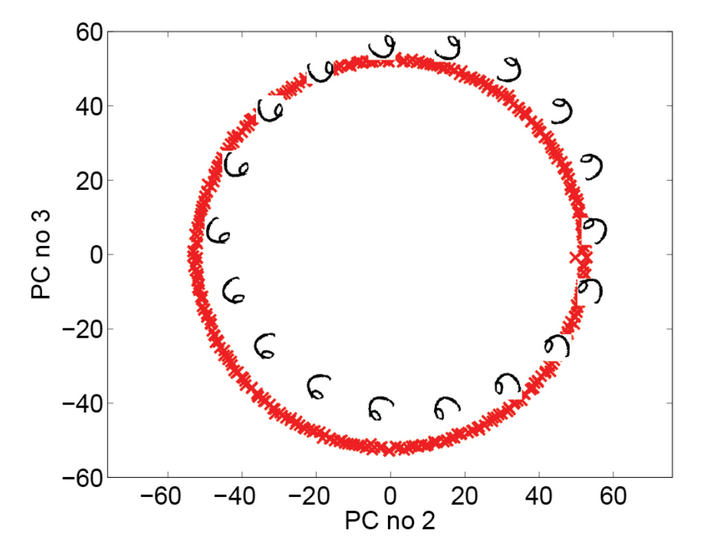
\includegraphics[width = 15cm]{images/DimRed/Manifold.png}
    \caption{Manifold that represents the rotation of a digit}
    \label{fig:manifold}
\end{figure}
This is usually possible for images since they have a structure and a semantic segmentation.

For data with structure we expect fewer distortions than dimensions and data usually live on a lower dimensional manifold. As a conclusion, we can deal with high dimensional data by looking for lower dimensional embeddings.

\subsubsection{PCA}
PCA is a method for dimension reduction that aims to maximize data variance after projection to some direction $u_{1}$. Projection points are:
\begin{equation} \label{projection}
    u_{1}^{T}x_{n}
\end{equation}
note that $u_{1}^{T}u_{1} = 1$

\begin{figure}[H]
    \centering
    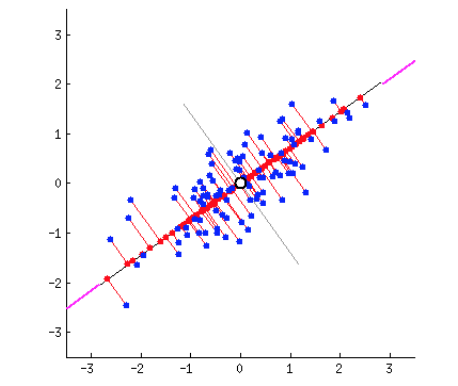
\includegraphics[width=10cm]{images/DimRed/pca.png}
    \caption{PCA variance maximization}
    \label{fig:pca}
\end{figure}

The first thing that we do is find the mean value of datapoints
\begin{equation}
    \overline{x} = \frac{1}{N}\sum_{n=1}^{N}x_n 
\end{equation}
and the data-centered matrix is:
\begin{equation}
    X=\begin{bmatrix}
    (x_{1} - \overline{x})^{T} \\ \dots \\ (x_{n} - \overline{x})^{T} \\ \dots \\ (x_{N} - \overline{x})^{T}
    \end{bmatrix}
\end{equation}
PCA is able to reduce \textbf{ONLY} to linear transformations. There are some techniques that are able to find non linear projections.
Now that data is normalized, we can find the linear projection that maximize the data. The projection point can be calculated as shown in \ref{projection}. If we apply the projection on every point, we have
\begin{equation}
    D = \langle u_{1}^{T}x_{n}, \dots, u_{1}^{T}x_{n}, \dots, u_{D}^{T}x_{n}\rangle
\end{equation}
now that we know how to apply the projection of points on a direction, we have to find which are the best directions. the mean of the projected points is $u_{1}^{T}\overline{x}$ and the variance of the projection points is:
\begin{equation}
\label{variance_of_projection}
    \frac{1}{N} \sum_{n=1}^{N}[u_{1}^{T}x_{n} - u_{1}^{T}\overline{x}]^{2} = u_{1}^{T}Su_{1}
\end{equation}
with
\begin{equation}
\label{cov_mat_norm}
    S = \frac{1}{N}\sum_{n=1}^{N}(x_{n} - \overline{x})(x_{n} - \overline{x})^{T} = \frac{1}{N}X^{T}X
\end{equation}
note: $S$ (\ref{cov_mat_norm}) is equal to the covariance normalized matrix, while \ref{variance_of_projection} is just a matrix multiplication on left and right of $S$ by $u_{1}$ (the left one is transposed).

If we try to maximize this value we get:
\begin{equation}
    \underset{u_{1}}{max}\ u_{1}^{T}Su_{1}
\end{equation}
subject to $u_{1}^{T}u_{1} = 1$. This is equivalent to unconstrained maximization with a Lagrange multiplier
\begin{equation}
    \underset{u_{1}}{max}\ u_{1}^{T}Su_{1} + \lambda_{1}(1 - u_{1}^{T}u_{1})
\end{equation}
and the solution is reached by setting the derivative w.r.t. $u_{1}$ to zero:
\begin{equation}
    Su_{1} = \lambda_{1}u_{1}
\end{equation}
where $u_{1}$ must be an eigenvector if $S$.

Left-multiplying by $u_{1}^{T}$ and using $u_{1}^{T}u_{1} = 1$, we have
\begin{equation}
    u_{1}^{T}Sy_{1} = \lambda_{1}
\end{equation}
which is the variance after the projection. In general, S will have different eigenvalues and eigenvectors. The eigenvalues that maximize the projections are the ones with an higher value. so, the first vector that will maximize the projection is the one associated to the highest eigenvalue, the second one will be the one associated to the second highest value, and so on.

\textbf{PCA Error minimization}: Consider a complete orthonormal D-dimensional basis such that
\begin{equation}
    u_{i}^{T}u_{j} = \delta_{ij}
\end{equation}
with
\begin{equation}
    \delta_{ij} =
    \begin{cases}
      1 \text{ if } i = j\\
      0 \text{ otherwise}
    \end{cases}
\end{equation}
Each datapoint can be written as 

\begin{equation}
    x_{n} = \sum_{i=1}^{d}\alpha_{ni}u_{i}
\end{equation}
using the orthonormal property we have $\alpha_{ni} = x_{n}^{T}u_{i}$, hence
\begin{equation}
    x_{n} = \sum_{i=1}^{d}(x_{n}^{T}u_{i})u_{i}
\end{equation}
the goal is to approximate $x_{n}$ using a lower-dimensional representation. We can write
\begin{equation}
    \Tilde{x}_{n} = \sum_{i=1}^{m}z_{ni}u_{i} + \sum_{i=m+1}^{d}b_{i}u_{i}
\end{equation}
Note: $b_{i}$ terms do not depend on sample $x_{n}$. \\
Evaluate approximation error (MSE) as
\begin{equation}
    J = \frac{1}{N}\sum_{n=1}^{N}||x_{n} - \Tilde{x}_{n}||^{2}
\end{equation}
Minimizing wrt $z_{nj}$ and $b_{i}$, we get:
\begin{equation}
    \begin{multlined}
        z_{ni} = x_{n}^{T}u_{i}\text{, } i= 1, \dots, m \\
        b_{i} = \overline{x}^{T}u_{i}\text{, } i= M + 1, \dots, d
    \end{multlined}
\end{equation}

Using these expression we get
\begin{equation}
    x_{n} - \Tilde{x}_{n} = \sum_{i=m+1}^{d} [(x_{n} - \overline{x})^{T}u_{i}]u_{i}
\end{equation}
The overall approximation error becomes
\begin{equation}
    J = \frac{1}{N}\sum_{n=1}^{N}\sum_{i=m+1}^{d}(x_{n}^{T}u_{i} - \overline{x}^{T}u_{i})^{2} = \sum_{i=m+1}^{d}u_{i}^{T}Su_{i}
\end{equation}

Minimize the approximation error subject to constraint $u_{i}^{T}u_{i} = 1$:
\begin{equation}
    \Tilde{J} = \sum_{i=m+1}^{d}u_{i}^{T}Su_{i} + \lambda_{i}(1 - u_{i}^{T}u_{i})
\end{equation}
If we set the derivative of a $u_{i}$ to zero, we get the exact same mathematical problem that we have found before:
\begin{equation}
    Su_{i} = \lambda_{i}u_{i}
\end{equation}
hence $u_{i}$ is an eigenvector of $S$ with eigenvalue $\lambda_{i}$. The approximation error is then given by:
\begin{equation}
    J = \sum_{i=m+1}^{d}\lambda_{i}
\end{equation}
and this is minimized by selecting $u_{i}$ as the eigenvectors corresponding to the $d - m$ smallest eigenvalues. In other words, the error is the sum of those last eigenvectors that we do not consider.

If we have less samples than dimensions, PCA is inefficient. a trick that we can use in this case is letting X be the $N\times d$ centered data matrix (i.e., n-th row is $(x_{n}-\overline{x})^{T}$) and the corresponding covarinace matrix:
\begin{equation}
    S = \frac{1}{N}X^{T}X
\end{equation}
the corresponding eigenvector equation is
\begin{equation}
    \frac{1}{N}X^{T}Xu_{i} = \lambda_{i}u_{i}
\end{equation}
By left multiplying by X we obtain:
\begin{equation}
    \frac{1}{N}XX^{T}(Xu_{i}) = \lambda_{i}(Xu_{i})
\end{equation}
and if we define $v_{i} = Xu_{i}$ we have
\begin{equation}
    \frac{1}{N}XX^{T}v_{i} = \lambda_{i}v_{i}
\end{equation}
so we have $XX^{T}$ which has the same $N - 1$ eigenvalues of $X^{T}X$ and is a $N\times N$ matrix whose eigenvalues can be computed efficiently.

given the eigenvalues $\lambda_{i}$ of $XX^{T}$, to find the eigenvectors we left-multiply by $X^{T}$
\begin{equation}
    \left(\frac{1}{N}XX^{T}\right)\left(X^{T}v_{i}\right) = \lambda_{i}\left(X^{T}v_{i}\right)
\end{equation}
This makes clear that $\left(X^{T}v_{i}\right)$ is an eigenvector of $S$ with eigenvalue $\lambda_{i}$. To find the direction $u_{i}$ we have to normalize the eigenvectors such that $u_{i}^{T}u_{i} = 1$:
\begin{equation}
    u_{i} = \frac{1}{\sqrt{N\lambda_{i}}} X^{T}v_{i}
\end{equation}

\textbf{Linear latent variable model}:
\begin{itemize}
    \item Represent data x with lower dimensional latent variables z
    \item Assume linear relationship $x = Wx + \mu$
    \item Assume Gaussian distribution of latent variables z $P(z) = N(z; 0, I)$
    \item Assume Linear-Gaussian relationship between latent variables and data $P(x|z) = N(x;Wz + \mu, \sigma^{2}I)$    
\end{itemize}
So, \textbf{Probabilistic PCA} is a model that, given the dataset, estimates the parameters of the models ($W, z$ and $\sigma$). we can setup a Maximum Likelihood that, given data $X$, sets the derivative of 
\begin{equation}
    \underset{W, \mu, \sigma^{2}}{argmax} \ln P(X|W, \mu, \sigma^{2}) = \sum_{n=1}^{N} \ln P(x_{n}|W, \mu, \sigma^{2})
\end{equation}
 to zero and finds the parameters of the model that, given z will generate a sample x.

\subsection{non-Linear Latent Variable Models}
Sometimes, linear representations are not sufficient for complex data
\begin{figure}
    \centering
    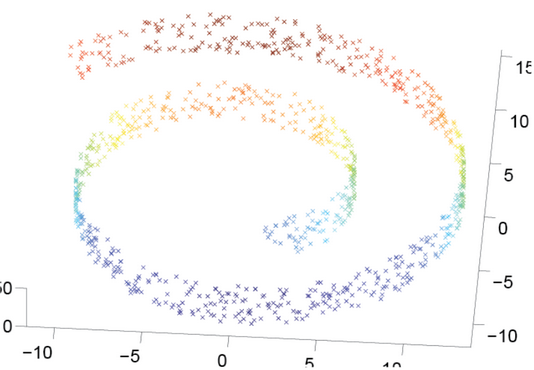
\includegraphics[width=8cm]{images/DimRed/non-linear-manifold.png}
    \caption{The ‘Swiss Roll’ dataset. 2D manifold embedded in 3D space.}
    \label{fig:non-linear-manifold}
\end{figure}

\subsubsection{Autoassociative Neural Networks (Autoencoders)}
An autoencoder is a combination of two Neural Networks: an encoder and a decoder. The train is based on reconstruction loss and provides a low-dimensional representation.

The structure is a neural network with a reduced size of hidden layers which learn to reconstruct their input by minimizing a loss function.
\begin{figure}[H]
    \centering
    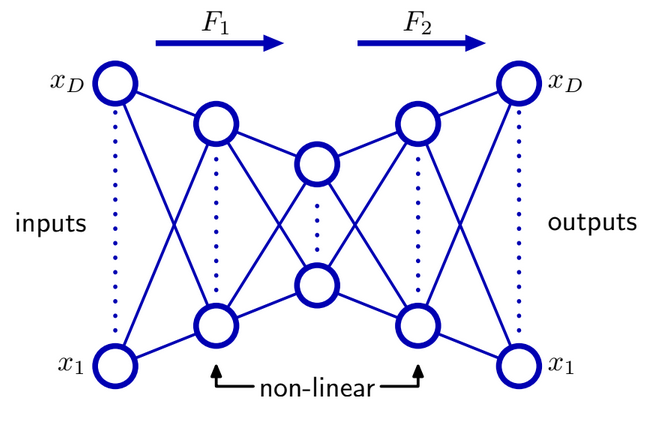
\includegraphics[width=8cm]{images/DimRed/autoencoder.png}
    \caption{A basic autoencoder example.}
    \label{fig:non-linear-manifold}
\end{figure}
It is important to have the same number of neurons in input and output.

We can also use autoencoders for image based application with Convolutional and Convolutional Transposed layers
\begin{figure}[H]
    \centering
    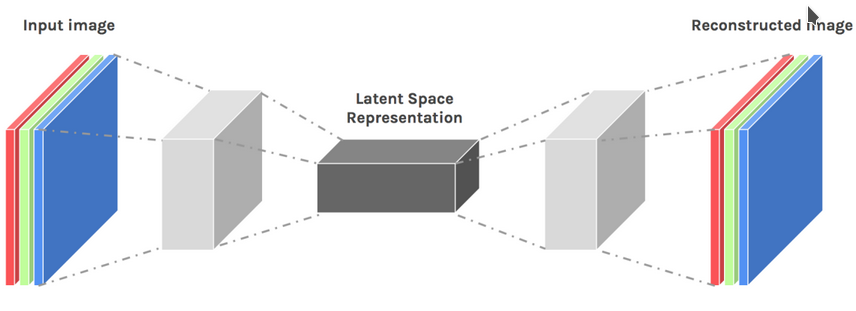
\includegraphics[width=8cm]{images/DimRed/autoencoder-image.png}
    \caption{Autoencoder for images.}
    \label{fig:non-linear-manifold}
\end{figure}
Given a dataset ${x_{n}}$, Autoencoders are trained with the same sample $x_{n}$ both in input and in output. Autoencoders learn how to encode/decode the samples in a dataset in a low-dimensional space. Autoencoders can be seen as a method for non-linear principal component analysis.

Autoencoders can be used for anomaly detection. We can teach an Autoencoder to reconstruct "good" samples and then calculate a threshold based on the final train loss found during training. We can then test samples, see if the reconstruction error is higher than the threshold and, if so, consider that sample an anomaly.

\subsection{Generative Models}
For these models, the aim is not only to reduce dimensionality, but also to use the latent space to reconstruct the input and modify it.

\textbf{Variational Auto-Encoders} (VAEs) focus on learning latent space structure\\
\textbf{Generative Adversal Networks} (GANs) focus on learning a distribution (no latent space in general)

\subsubsection{VAEs}
The goal is to modify the data in specific directions and identify meaningful directions in latent space. Some examples are face distortion, digit production and 3D mesh distortion.

\begin{figure}[H]
    \centering
    \begin{subfigure}[b]{0.45\textwidth}
        \centering
        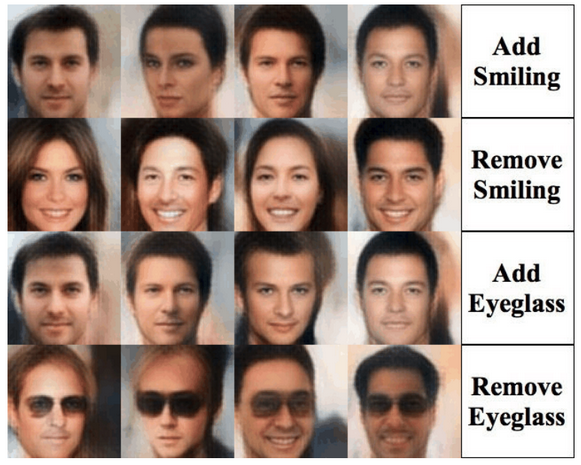
\includegraphics[width=\textwidth]{images/DimRed/vaes-1.png}
        \caption{Example of application of VAEs on faces.}
        \label{fig:vaes_1}
    \end{subfigure}
    \hfill
    \begin{subfigure}[b]{0.45\textwidth}
        \centering
        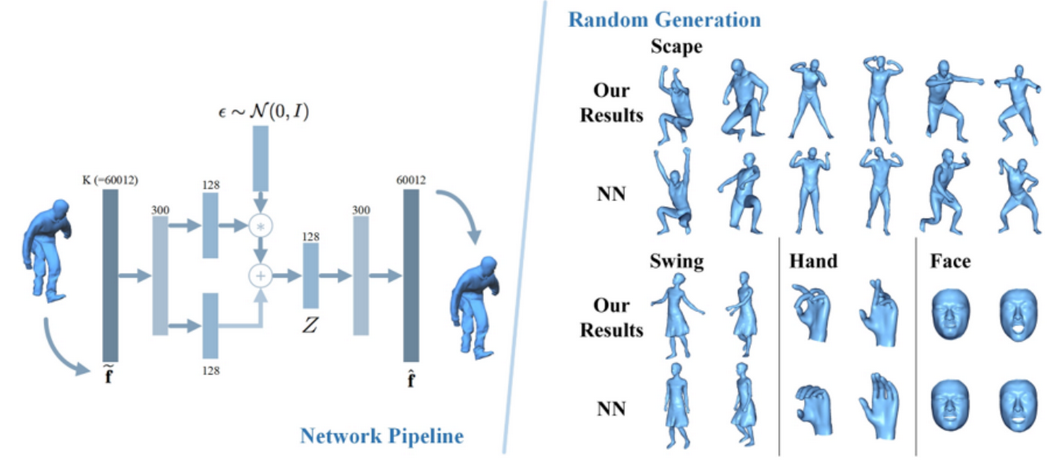
\includegraphics[width=\textwidth]{images/DimRed/vaes-2.png}
        \caption{Example of application of VAEs on 3D mesh fold.}
        \label{fig:vaes_2}
    \end{subfigure}
\end{figure}

Main idea: Encoder produces a distribution instead of a vector. Decoder operates on samples from this distribution

\begin{figure}[H]
    \centering
    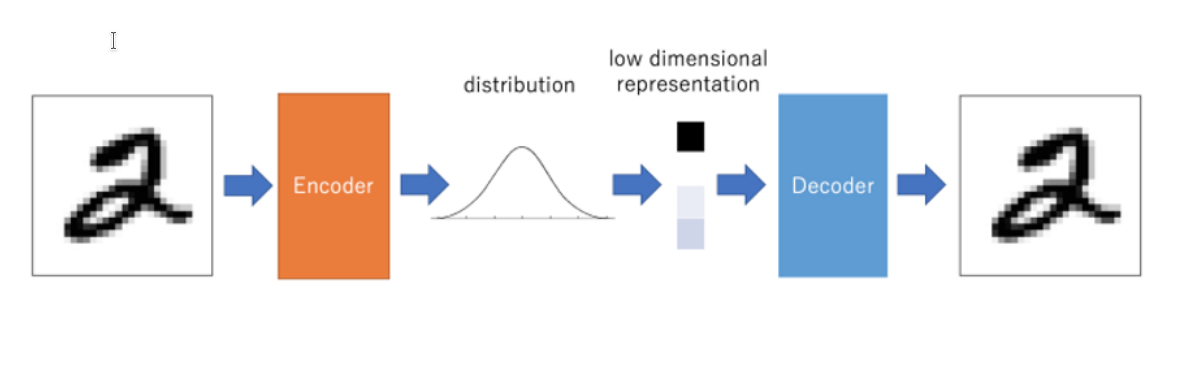
\includegraphics[width=12cm]{images/DimRed/vae.png}
    \caption{VAE architecture.}
    \label{fig:non-linear-manifold}
\end{figure}

But how do we produce a distribution? How do we prevent degeneration? We can consider a parametric distribution (typically Gaussian that produces a mean and a variance). Then we add a loss term based on the KL divergence (Evidence Lower Bound) that gives how much the distribution of the latent space differs from a standard Gaussian distribution with 0 mean and an identity covariance matrix. We also have another factor $\epsilon$ that works as a weight and regulates the strictness of the re-parametrization of the Gaussian that the VAE is learning (an high $\epsilon$ brings better looking Gaussians but worsen the reconstruction quality).

In practice, since we have a distribution, we could try to sample one value of the distribution. For instance, if we have an image and we give it to the decoder of a VAE, we get a value as output. Then, the value is processed by the Gaussian distribution and this generates a sample. This sample is then passed to the decoder who generates the output.

The sampling operation is easy to perform forward given the parameters of the Gaussian. However, if we have to compute the gradient for the backpropagation, and the sampling operation is not invertible. We then solve this problem by introducing the concept of generating a sample during backpropagation and sum this value to the output of the encoder. Since this can be treated just like a constant value, during backpropagation we know how to derive it and so we can proceed.

\subsubsection{GANs}

The main goal is to sample from the input data distribution $X$. The idea is based on inverting a CNN and use adversal training. 

A GAN firstly has an encoder that uses a CNN to process an image and transform it into a vector. Following, a Decoder receives a code and produces an image. This second element uses a "deconvolutional" operator.

What we then want to do is being able to use only the decoder so that, if we give a vector as input, it is able to reconstruct an image. The meaning of dimensionality reduction is loosing importance and what really matters is the generation of an image from a vector.

now the problem becomes: How to train the decoder to produce meaningful data? 

Adversal training is when two parts of the network are competing each other in order to find an optimal solution. In GANs, we use adversal training to improve reconstruction. A GAN is then a combination of two networks: the generator network (or decoder) and the discriminator network (or critic).

The Discriminator can take as input both  real images from the dataset and images sampled from the generator. He then has to decide if the input is a real or a fake image.

\begin{figure}[H]
    \centering
    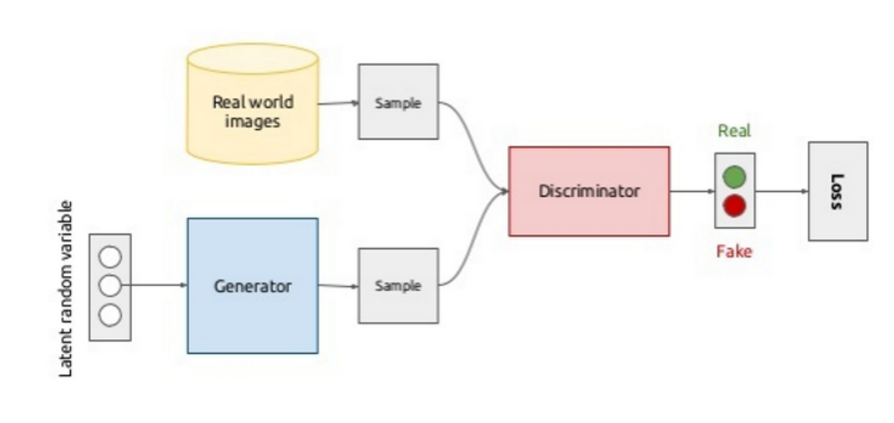
\includegraphics[width=12cm]{images/DimRed/GAN.png}
    \caption{GAN architecture.}
    \label{fig:non-linear-manifold}
\end{figure}

So, there are two roles in a GAN:
\begin{itemize}
    \item Generator produces samples of the distribution $P(X)$
    \item Discriminator identifies if a sample actually comes from the (unknown) $P(X)$ or not
\end{itemize}

during training procedure, we have the networks competing with each other:
\begin{itemize}
    \item generator tries to fool the discriminator in believing that the sample is ‘real’
    \item discriminator tries to discriminate as good as possible ‘real’ from ‘fake’ samples
\end{itemize}

and the training steps are:
\begin{enumerate}
    \item Train the discriminator by keeping the generator fixed. During this phase, images from the generator are labeled as fake because the discriminator has to learn the difference between fake and real images.
    
    \vspace{0.1cm}
    
    AKA. Train the discriminator with a batch of data $\{(x_{n}, \text{Real})\} \cup {(x_{m}', \text{Fake})}$, where $x_{n}$ comes from the data set, while $x_{m}'$ are images generated from the generator with random values of the latent variable.
    \item Train the generator by keeping the discriminator fixed. During this phase, images from the generator are labeled as real because the generator wants to fool the discriminator.
    
    \vspace{0.1cm}
    
    AKA. Train the generator by using the entire model (generator + discriminator) with discriminator layers fixed (i.e., not trainable) with a bacth of data ${(r_{k}, \text{Real})}$, where $r_{k}$ are random values of the latent variable
\end{enumerate}

What about the loss? We can notice that when the loss increases for the discriminator, it decreases for the generator and viceversa. Very often, if you plot the losses during time it will have a 2d-DNA shape that slowly decreases until they will converge. We don't want to have that one of the two losses goes to zero while the other diverges. A model is trained when the two losses converge and the accuracy of the discriminator is around 50\%. Now we can generate images from the generators that are similar to the ones from the dataset.

Additional topic: GANs can be exploited to attack ML models !!! A generative model can be defined in order to make an anomaly detection model fail.